\clearpage
\setcounter{section}{0}
\renewcommand{\thesection}{H.\arabic{section}}
\renewcommand{\theHsection}{annexH.\arabic{section}}

\phantomsection
\addcontentsline{toc}{chapter}{Annexure H: Criteria 8 Supporting Documents}
\label{app:criteria-8}

\refstepcounter{section}
\phantomsection
\label{app:cqi}
\addcontentsline{toc}{section}{\protect\numberline{\thesection}Rejoinder}

% ---- Heading block ----
\newcommand{\annexHFirstPageHead}{%
  \noindent{\Huge\bfseries Annexure H: Criteria 8 Supporting Documents}\par
  \vspace{0.8em}
  \noindent Here we provide the supporting annexures required for Criterion 8: Continuous Quality Improvement (CQI).\par
  \vspace{0.8em}
  \noindent{\Large\bfseries\thesection\quad Rejoinder}\par
  \vspace{0.5em}
}

% Display the heading before the table
\annexHFirstPageHead
This rejoinder presents the responses and clarifications provided by the Software Engineering Department at SEECS to the observations and recommendations arising from the previous accreditation review under Criterion 8: Continuous Quality Improvement (CQI). It summarizes the actions taken to address the identified issues, the improvements implemented, and the measures adopted to strengthen continuous quality improvement practices within the programme. The rejoinder is supported by relevant documentary evidence, presented in the following table, to facilitate verification of the responses and the progress achieved.
\begin{landscape}
\label{annex:rejoinder}
\scriptsize

\begin{longtable}{|P{2.3cm}|P{5.0cm}|P{4.5cm}|P{5.0cm}|P{2.4cm}|P{2.8cm}|P{1.8cm}|}
\hline
\rowcolor{gray!25}
\textbf{Criteria} & \textbf{PEC Observation} & \textbf{Root Cause Analysis} & \textbf{Corrective Action Plan} & \textbf{Implementation Status} & \textbf{Evidence} & \textbf{Reference to SAR} \\
\hline
\endfirsthead
\hline
\rowcolor{gray!25}
\textbf{Criteria} & \textbf{PEC Observation} & \textbf{Root Cause Analysis} & \textbf{Corrective Action Plan} & \textbf{Implementation Status} & \textbf{Evidence} & \textbf{Reference to SAR} \\
\hline
\endhead

\multirow{2}{=}{\textbf{PEO}} & The process for assessing the achievement of Program Educational Objectives (PEOs) is clear. Key Performance Indicators (KPIs) are well-defined, and assessment tools are in use. However, there is a noticeable lack of correlation in the survey forms used to assess certain sub-KPIs related to PEO-2 and PEO-3. The cumulative KPI attainment process is well-documented in the approved policy. & The observation regarding the lack of correlation between certain survey items and the sub-KPIs of PEO-2 and PEO-3 is acknowledged. On review of the existing alumni and employer survey forms, the Department confirmed this concern and further noted that some questions were vaguely framed and that the PEOs were assessed through an uneven number of questions. & The Department undertook a review activity and comprehensively revised both the alumni and employer survey forms. In the revised questionnaires, each question is directly aligned to a specific PEO, ambiguity has been removed, and every PEO is now measured through an equal number of questions to ensure balanced and valid attainment. & Complete & Alumni \& Employer Survey Forms & Sec.~\ref{revised-assesment-instrument}; Annex~\ref{app:revised forms}, \ref{annex:alumni}, \ref{annex:employer} \\ \hline
 & The Continuous Quality Improvement (CQI) process at the Program Educational Objectives (PEO) level has been initiated. Some assessment data has been collected using existing survey forms, and analysis and evaluation have been conducted. Stakeholder feedback is also gathered for the revision of survey forms. Corrective actions have been identified, but there are issues with the implementation of these actions. & Although PEO assessment data and stakeholder feedback were being collected, the Department lacked a structured mechanism to systematically implement, monitor, and document corrective actions arising from the evaluation results. In addition, the PEO assessment methodology and survey instruments required further refinement to support effective CQI implementation. & Comprehensively revise the stakeholder survey instruments, improve the PEO KPI evaluation mechanism through a structured assessment methodology, and incorporate Industrial Advisory Board feedback to strengthen the PEO assessment and review process. & Complete & IAB Meeting Minutes, Evaluation System mentioned in Criteria 1 & Sec.~\ref{attainment-of-peos}, \ref{attainment-results}, \ref{program-improvement}, \ref{subsec:new-peo-evaluation-framework}; Annex~\ref{app:iab_feedback_full}, \ref{app:iab_minutes} \\ \hline
\multirow{4}{=}{\textbf{PLO}} & The department has updated the Program Educational Outcomes (PEOs), but it appears that some essential elements of PEO-2 are not addressed in the Program Learning Outcomes (PLOs). & During the review of the PEO–PLO alignment, it was identified that the mapping did not explicitly capture the "innovative solution development" component of PEO-2. Although PLO-8, PLO-9, and PLO-10 addressed leadership, teamwork, communication, and project management, the design and innovation aspect was omitted from the mapping. & The PEO–PLO mapping was reviewed and revised to explicitly align PEO-2 with PLO-3 (Design/Development of Solutions) in addition to PLO-8, PLO-9, and PLO-10. The updated mapping ensures comprehensive coverage of leadership, teamwork, communication, project management, and innovative solution development within PEO-2. & Complete & Updated Mapping available in Crteria 2 of SAR & Sec.~\ref{sec:plopeo}; Annex~\ref{app:criteria-2_plo-peo_mapping_rationale} \\ \hline
 & The course-to-PLO mapping demonstrates satisfactory alignment with all PLOs. Nevertheless, there are notable weaknesses in the mapping, particularly concerning PLO-3 and PLO-1, in terms of the learning domain and taxonomy level. However, the department has provided data regarding the ongoing mapping revision for upcoming semesters, which is based on Continuous Quality Improvement (CQI) and utilizes the course review performa. & The review identified that the CLOs of certain courses were not optimally aligned with the intended learning domains and Bloom's Taxonomy levels of PLO-1 and PLO-3. As a result, the course-to-PLO mapping did not fully reflect the required cognitive complexity and expected outcome attainment. & Implemented a comprehensive review and revision of course specifications, including refinement of CLOs, updating Bloom's Taxonomy levels and learning domains, and revising the course-to-PLO mapping through the departmental CQI process based on Course Review Reports, faculty discussions, and DBS recommendations. & Completed & CLO-PLO Mapping available in Criteria 2 & Sec.~\ref{sec:cloplo}; Annex~\ref{OBE Assessment Configuration on Qalam} \\ \hline
 & Assessment methodologies, including both direct and indirect methods, are established. However, the assessment methods for achieving PLOs through indirect means need improvement, especially in the case of the poorly designed internship form and the graduate exit survey forms. Furthermore, although direct assessment methods are in use, they are not consistently applied in certain instances for a couple of PLOs, specifically PLO-8 and PLO-10. & The review identified that the Internship Employer Feedback Form and Graduate Exit Survey Form were not adequately aligned with the Program Learning Outcomes and lacked well-defined assessment indicators for reliable indirect assessment. In addition, direct assessment of PLO-8 and PLO-10 was not consistently integrated into the CLOs and assessment instruments of relevant courses. & The Internship Employer Feedback Form and Graduate Exit Survey Form were comprehensively revised to improve clarity, incorporate well-defined PLO-based assessment indicators, and strengthen indirect assessment. An online Internship Feedback Module was integrated with the Thesis Management System (TMS) to institutionalize employer feedback collection and reporting. Additionally, the direct assessment methodology was reviewed and updated by revising CLO-to-PLO mappings and course specifications to ensure consistent assessment of all PLOs, including PLO-8 and PLO-10, through appropriate assessment instruments. & Complete & Internship Feedback Form \& Graduate Exit Survey Form and CLO-PLO Mapping & Sec.~\ref{sec:indirectassess}, \ref{revised-assesment-instrument}, \ref{subsec:new-internship-mechanism}, \ref{sec:cloplo}; Annex~\ref{annex:internship-feedback-form}, \ref{annex:internship-feedback-analysis}, \ref{annex:graduate-exit-survey-form}, \ref{annex:graduate-exit-survey-analysis} \\ \hline
 & The Key Performance Indicators (KPIs) are clearly defined. However, there is an issue with the assessment process in direct assessment, as it is not consistently conducted at the appropriate taxonomy level. Additionally, the quality of the assessment process in the case of indirect methods appears to be subpar, especially when using the internship feedback form. & The review identified that the assessment instruments of some courses were not consistently aligned with the intended Bloom's Taxonomy levels defined for the CLOs, resulting in inconsistencies in direct assessment. Additionally, the existing Internship Employer Feedback Form lacked well-defined PLO-based assessment indicators and a structured mechanism for systematic data collection and analysis, reducing the effectiveness of indirect assessment. & Conducted a comprehensive review and revision of course specifications, including CLOs, Bloom's Taxonomy levels, and assessment instruments, to ensure direct assessment is performed at the intended cognitive level and aligned with the relevant PLOs. The Internship Employer Feedback Form was comprehensively redesigned with improved PLO-based assessment indicators, and an Online Internship Feedback Module integrated with the Thesis Management System (TMS) was implemented to institutionalize employer feedback collection, reporting, and analysis, thereby improving the reliability, consistency, and traceability of indirect assessment data. & Indirect assesment method Complete, Continuously improving mappings through CQI Cycles & Internship Feedback Form, Course Outlines for Information Security \& Software Design \& Architecture & Sec.~\ref{revised-assesment-instrument}, \ref{subsec:new-internship-mechanism}, \ref{sec:cloplo}; Annex~\ref{annex:internship-feedback-form} \\ \hline
\multirow{5}{=}{\textbf{Curriculum}} & The department has supplied a list of courses that cover CEP attributes. The visitation team has been presented with data related to CEPs and their assessments. However, the visitation team has observed a lack of understanding in the assessment of CEPs, along with identified weaknesses concerning the clarity and complexity level of CEP attributes in statements provided, particularly in a few courses. & The review identified that faculty members had varying levels of understanding regarding the formulation, mapping, and assessment of Complex Engineering Problem (CEP) attributes. In addition, the absence of standardized guidelines resulted in inconsistencies in the clarity and cognitive complexity of CEP statements across a few courses. & Conducted dedicated faculty training sessions on the formulation, mapping, and assessment of CEP attributes in accordance with PEC guidelines. A standardized CEP template, along with illustrative examples, was developed and disseminated to all course instructors to ensure consistent formulation, appropriate complexity levels, and uniform assessment of CEP attributes across courses. & Complete & CEP Training List, CEP Guidelines & Sec.~\ref{sec:4.2cep}, \ref{subsubsec:cep-oel}; Annex~\ref{app:criteria-3_CEP Policy for BESE Department}, \ref{app:criteria-3_CEP Example} \\ \hline
 & The use of rubrics-based assessment mechanisms in the lab is evident, as observed from the lab folders and during the visit to the labs. However, it is noted that the assessment mechanisms, especially in the Psychomotor and Affective domains, are not appropriate in certain lab courses, such as operating systems and deep learning. The visitation team also observed inconsistencies in the experiments included in the lab folders of a few courses, like Computer Architecture and Logic Design, where the experiments did not align with the course contents as per the syllabus. & The department's Continuous Quality Improvement review identified opportunities to further refine laboratory assessment practices and standardize laboratory content to ensure consistent alignment with the approved course syllabi, intended learning outcomes, and Bloom's Taxonomy levels. & Conducted dedicated training sessions for faculty members and lab engineers on the design of open-ended lab exercises and rubric-based assessment of the Psychomotor and Affective domains. In addition, a standardized laboratory manual template was developed and implemented across the Software Engineering Department to ensure consistency in laboratory content, alignment with approved course outlines, and uniform assessment practices. The laboratory assessment rubrics and manuals were also reviewed to ensure appropriate alignment with the intended learning outcomes and Bloom's Taxonomy levels. & Complete & OEL Training, Standardized Template, Rubrics Sample & Sec.~\ref{sec:labrubrics}, \ref{sec:labassessment}, \ref{subsubsec:cep-oel}; Annex~\ref{app:criteria-3_Sample Lab Manual}, \ref{app:criteria-3_Lab Rubric Based Evaluation}, \ref{app:criteria-3_Sample Open Ended Lab} \\ \hline
 & Course Learning Outcomes (CLOs) are defined for all courses, but the visitation team has identified issues with the taxonomy levels and their mapping to relevant Program Learning Outcomes (PLOs) in many course outlines. This discrepancy is notably observed in courses like Design and Analysis of Algorithms and Operating Systems etc. & The department's periodic review of course specifications identified opportunities to further refine the formulation of Course Learning Outcomes (CLOs) and strengthen their alignment with the intended Bloom's Taxonomy levels, learning domains, and corresponding Program Learning Outcomes (PLOs) in a few courses. & Conducted a comprehensive review and revision of course specifications through the departmental CQI process. Course Learning Outcomes were refined to improve clarity and measurability, Bloom's Taxonomy levels and learning domains were updated where required, and course-to-PLO mappings were revised based on Course Review Reports, faculty deliberations, and Departmental Board of Studies (DBS) recommendations. The revised course specifications have been implemented in the current curriculum to ensure appropriate cognitive complexity and improved alignment with the intended PLOs. & Complete & CLO-PLO Mapping available in Criteria 2 & Sec.~\ref{sec:cloplo}, \ref{sec:4.10assessment}; Annex~\ref{app:criteria-3_Course Outline with Knowledge Group Head's Signature} \\ \hline
 & Assessment in the knowledge domain is generally appropriate, but at times it lacks rigor, as evident from the course folders, particularly in courses like Operating System, Organizational Behavior, and Computer Architecture and Logic Design. The assessments in the Psychomotor and Affective domains also require significant improvement for the evaluation of Course Learning Outcomes (CLOs) and Program Learning Outcomes (PLOs). Additionally, it was noted that rubrics are not consistently followed for assessment in the Affective domain in some courses, specifically those mapped to PLO-10. & The department's periodic review identified opportunities to further enhance the consistency and rigor of assessment instruments across a few courses, particularly in strengthening the evaluation of the Psychomotor and Affective domains and ensuring the uniform application of rubric-based assessment for courses mapped to PLO-10. & Conducted dedicated Outcome-Based Education (OBE) training sessions for faculty members of the Humanities and Sciences Department, who primarily offer courses mapped to PLO-8 and PLO-10, to strengthen their understanding of rubric-based assessment, appropriate CLO coverage, and alignment with Bloom's Taxonomy levels. Faculty members were also instructed to develop and include assessment rubrics for every Psychomotor and Affective domain assessment to ensure consistent, transparent, and outcome-based evaluation. These initiatives have enhanced the quality, consistency, and rigor of assessment practices across the relevant courses. & Complete & H\&S Training Minutes \& Feedback, Rubrics Sample for Affective Domain & Sec.~\ref{sec:labrubrics}, \ref{subsec:faculty-development-training}, \ref{criterion-8-review-and-corrective-action-processes-for-clos}; Annex~\ref{app:criteria-3_Lab Rubric Based Evaluation} \\ \hline
 & Satisfactory attainment is observed in all three domains. However, the visitation team noted that in several courses (e.g., Design and Analysis of Algorithms, Software Design and Architecture, Formal Methods, Internet of Things, etc.), assessments for Course Learning Outcomes (CLOs) are conducted at a lower taxonomy level. This should be addressed through Continuous Quality Improvement (CQI). It is also worth mentioning that despite the lower taxonomy levels, the assessment appears to be at a suitable level of complexity, indicating a potential lack of faculty understanding about taxonomy levels. This is an area that requires improvement. & The department's periodic review identified opportunities to further strengthen the consistency between the documented Bloom's Taxonomy levels of certain Course Learning Outcomes (CLOs) and the cognitive complexity of the corresponding assessment instruments. The review also highlighted the need for greater consistency in the application of Bloom's Taxonomy during course design and assessment planning. & Conducted a comprehensive review of the affected course specifications through the departmental CQI process and revised the Course Learning Outcomes (CLOs), Bloom's Taxonomy levels, and course-to-PLO mappings to accurately reflect the intended cognitive complexity of the assessments. Faculty awareness of Bloom's Taxonomy was further strengthened through curriculum review meetings and internal OBE discussions to promote the consistent application of taxonomy levels during course design, assessment planning, and periodic course reviews. & Complete & CLO-PLO Mappin, CQI cycle for CLO revision samples & Sec.~\ref{sec:cloplo}, \ref{sec:cqiclos}, \ref{criterion-8-review-and-corrective-action-processes-for-clos}; Annex~\ref{annex:caf-oop}, \ref{annex:dbs-mom}, \ref{annex:oop} \\ \hline
\multirow{2}{=}{\textbf{Faculty \& Support Staff}} & There is a formal training mechanism in place for faculty development; however, it has been noted that this mechanism does not comprehensively cover all areas, particularly those related to learning domains and taxonomy levels. & The department's review identified an opportunity to further strengthen and formalize faculty development activities related to Outcome-Based Education (OBE), particularly in the consistent application of learning domains, Bloom's Taxonomy levels, and constructive alignment during course design and assessment. & Strengthened the departmental faculty development mechanism by institutionalizing dedicated OBE training for newly inducted faculty through the NNUST Certificate for Teaching \& Learning (NCTL) and conducting regular refresher workshops at the department and SEECS levels. The training covers the formulation of measurable CLOs, selection of appropriate learning domains and Bloom's Taxonomy levels, CLO–PLO mapping, design of aligned assessment instruments, and constructive alignment of teaching, learning, and assessment. Faculty participation in national and international professional development programs has also been encouraged to further enhance pedagogical and technical competencies. & Repeated at Regular Intervals & Training List & Sec.~\ref{sec:training}, \ref{subsec:faculty-development-training} \\ \hline
 & Most of the teaching staff in the department are in the early stages of their academic careers, with a significant number being junior faculty members. & The department's faculty expansion in recent years has included the recruitment of talented early-career academics to support program growth and future capacity building. To ensure consistency in academic quality and Outcome-Based Education (OBE) practices, structured mentoring and professional development were identified as key enablers for faculty development. & Maintained a balanced faculty profile in which more than 60\% of the faculty members possess around 10 years or more of academic and/or industry experience, providing strong academic leadership and mentoring. Strengthened the faculty development framework by implementing structured induction and mentoring programs for newly inducted faculty, including mandatory OBE training through the NUST Certificate for Teaching \& Learning (NCTL), supervised teaching, and continuous professional development activities. Junior faculty members were paired with experienced mentors to support curriculum delivery, assessment practices, research supervision, and adherence to departmental quality assurance processes, ensuring continuity and sustained academic excellence. & Repeated at Regular Intervals & Faculty List available in Chapter 5 & Sec.~\ref{faculty-strength-and-competencies}, \ref{sec:training}; Annex~\ref{annex:I}, \ref{annex:J} \\ \hline
\multirow{1}{=}{\textbf{Facilities and Infrastructure}} & The library has successfully acquired a substantial collection of books; however, it is currently facing budget-related constraints that need to be addressed in order to accommodate future growth. In addition to traditional resources, digital library resources are also available. It's worth noting that the library software is accessible, offering the potential for efficient resource management and organization once access issues are resolved. Efforts to expand physical space, address system-related challenges, and optimize the library software will greatly enhance the overall library experience for students and faculty, enabling seamless access to a wide range of educational resources. & The NUST Library System provides a comprehensive collection of print and digital resources supported by established library management processes and periodic institutional reviews. As part of its continuous enhancement approach, these reviews identified opportunities to further optimize library services, digital resource accessibility, library management systems, and learning spaces to better support the evolving academic and research requirements of students and faculty. & Strengthened library services through continuous enhancement of the Central Library facilities, regular maintenance and upgrading of the KOHA Integrated Library Management System and DSpace Institutional Repository, and ongoing coordination with the ICT Directorate to improve network reliability and access to electronic resources. Expanded access to national and international digital resources, including the HEC Digital Library and major scholarly databases, while continuously updating the Institutional Repository with research publications and theses. Future enhancement initiatives have also been planned, including expansion of seating capacity, improved collaborative learning spaces, dedicated research commons, and AI-enabled library support services. & In-Process &  & Sec.~\ref{library}, \ref{Digital ibrary}, \ref{library statistics}, \ref{subsubsec:network-connectivity} \\ \hline
\multirow{4}{=}{\textbf{CQI}} & The CQI (Continuous Quality Improvement) process is in place and being practiced at all levels. However, the actual implementation of the CQI policy on the ground suggests that some corrective actions have not been taken, or implementation plans are still in progress, particularly in regard to PEO (Program Educational Objectives), Course Mappings, and Taxonomy Levels. & The department's periodic CQI review identified opportunities to further strengthen the implementation and documentation of corrective actions, particularly in relation to PEO evaluation, course mappings, and the alignment of Course Learning Outcomes (CLOs) with the appropriate learning domains and Bloom's Taxonomy levels. & Implemented comprehensive revisions to the PEO evaluation survey instruments, updated Course Learning Outcomes (CLOs), learning domains, Bloom's Taxonomy levels, and course-to-PLO mappings through the departmental CQI process, and strengthened the internship evaluation process by introducing improved assessment instruments. In addition, regular faculty training and periodic course reviews have been institutionalized to ensure the consistent implementation, monitoring, and continuous enhancement of Outcome-Based Education (OBE) practices. & Completed & Survey Forms and CQI Cycle Samples & Sec.~\ref{revised-assesment-instrument}, \ref{criterion-8-corrective-actions-for-curriculum}, \ref{criterion-8-review-and-corrective-action-processes-for-clos}, \ref{subsec:cqi-obe-system-enhancements}; Annex~\ref{app:revised forms}, \ref{annex:caf-oop}, \ref{annex:oop} \\ \hline
 & Only partial actions have been taken, and the implementation plans are unsatisfactory. The concerns and weaknesses identified in the last accreditation visit report, particularly in Criterion 2, 3, and 8, still require comprehensive and dedicated attention. & The department's review of the previous accreditation recommendations identified opportunities to further strengthen the implementation, monitoring, and documentation of Continuous Quality Improvement initiatives, particularly for Outcome-Based Education processes under Criteria 2, 3, and 8. & To strengthen the departmental CQI system, a dedicated Departmental CQI Committee was constituted following the previous PEC accreditation visit to oversee the planning, implementation, monitoring, and documentation of continuous improvement initiatives. The Committee has institutionalized the periodic review of Course Learning Outcomes (CLOs), CLO–PLO mappings, assessment results, and stakeholder feedback to identify and implement evidence-based corrective actions. In addition, the department implemented an autonomous online internship feedback system, redesigned the Graduate Exit Survey using outcome-oriented indicators, and conducted regular faculty capacity-building sessions on Outcome-Based Education (OBE). These initiatives have significantly strengthened the implementation and sustainability of the department's CQI processes. & Repeated at Regular Intervals & CQI Committee Formation & Sec.~\ref{local-quality-enhancement-cell-lqec}, \ref{subsec:cqi-obe-system-enhancements} \\ \hline
 & There is a significant number of journal publications, and senior faculty members are actively involved in funded research and development projects. However, it's noteworthy that only one faculty member is engaged in consultancy activities. & The department's periodic review identified opportunities to further strengthen faculty engagement with industry through consultancy activities while continuing to promote excellence in research, innovation, and externally funded projects. & Strengthened institutional support for faculty consultancy by encouraging industry engagement, facilitating consultancy opportunities, and promoting faculty participation in collaborative projects with industry. The department also continued to support faculty research through research funding, faculty placement programs, incentives for innovation and spin-off ventures, and other research development initiatives. As a result, multiple faculty members are now actively engaged in consultancy activities, in addition to their research and development contributions. & On-going & Consultanies List, Faculty Placement Evidence & Sec.~\ref{sec:c9-faculty-placement}, \ref{sec:c9-consultancy}; Annex~\ref{app:post} \\ \hline
 & A limited number of new initiatives have been undertaken. Moreover, the implementation of OBE (Outcome-Based Education) requires improvements in the assessment and evaluation processes. & The department's Continuous Quality Improvement review identified opportunities to further strengthen Outcome-Based Education (OBE) implementation by introducing additional quality enhancement initiatives and reinforcing the consistency of assessment and evaluation processes. & Implemented multiple initiatives to strengthen OBE, including the introduction of an autonomous online internship feedback system, revision of indirect assessment instruments, periodic review of Course Learning Outcomes (CLOs) and CLO–PLO mappings, and systematic analysis of assessment results through the Departmental CQI Committee. Regular OBE training and capacity-building sessions have been conducted for faculty, while all assessment instruments are reviewed by the respective Knowledge Group Heads to ensure alignment with defined CLOs, appropriate Bloom's Taxonomy levels, and the principles of Outcome-Based Education. Assessment results are analyzed at the end of each semester, and evidence-based corrective actions are implemented to support continuous enhancement of assessment and evaluation practices. & On-going & CQI Cycle Samples & Sec.~\ref{sec:cqiclos}, \ref{subsec:cqi-obe-system-enhancements}; Annex~\ref{annex:caf}, \ref{annex:caf-oop}, \ref{annex:oop}, \ref{annex:dbs-mom} \\ \hline
\multirow{3}{=}{\textbf{Industrial Linkages}} & Both formal and informal mechanisms are in place; however, there is a need for the assessment tools and methods to have a stronger correlation with the Program Educational Objectives (PEOs). & The department's review identified opportunities to strengthen the alignment of indirect assessment tools with the Program Educational Objectives (PEOs) to improve the reliability and traceability of evidence used for PEO evaluation. & Institutionalized the collection of employer feedback through a dedicated Online Internship Feedback Module integrated with the Department's Thesis Management System (TMS). The revised employer feedback mechanism enables systematic collection, storage, and analysis of assessment data aligned with the Program Educational Objectives (PEOs), supports the generation of consolidated batch-wise reports, and enhances the reliability, traceability, and evidence-based Continuous Quality Improvement (CQI) of the PEO assessment process. & Complete &  & Sec.~\ref{sec:c9-industrial-feedback}, \ref{subsec:new-internship-mechanism}, \ref{subsec:new-peo-evaluation-framework}; Annex~\ref{app:revised forms} \\ \hline
 & There are projects that are jointly supervised by the industry, but there is no substantial evidence of sponsored design projects from the industry. & The department's review identified opportunities to further expand formal industry-sponsored Final Year Design Projects (FYDPs) by strengthening structured collaborations with industry partners beyond the existing practice of joint industry supervision. & Strengthened industry engagement by actively pursuing formal collaborations with industry through Memoranda of Understanding (MoUs), funded industry partnerships, and collaborative research and development initiatives to increase the number of industry-sponsored Final Year Design Projects (FYDPs). The department has also enhanced its engagement with industrial partners to facilitate sponsored projects for future cohorts while continuing the practice of joint industry supervision. & On Going & List of Industry Funded Projects & Sec.~\ref{sec:c9-design-projects}, \ref{sec:c9-industry-collab}, \ref{subsec:industry-linkages-partnerships}; Annex~\ref{annex:industryproj} \\ \hline
 & Taking into account the overall faculty strength, there is limited faculty involvement observed in engaging in projects and providing consultancy services to the industry. & The department recognized the need to further strengthen faculty interaction with industry by expanding participation in consultancy, collaborative research, and industry-sponsored projects to complement its academic and research excellence. & Initiated measures to strengthen faculty engagement with industry by promoting consultancy assignments, collaborative research and development (R\&D), and industry-sponsored projects. The department has enhanced partnerships with industry, introduced facilitation mechanisms to support faculty-industry collaboration, and encouraged participation through institutional incentives. These initiatives have established a stronger framework for increasing faculty involvement in consultancy and applied industrial projects. & On Going & List of Consultancies & Sec.~\ref{sec:c9-consultancy}, \ref{sec:c9-industry-collab} \\ \hline
\end{longtable}
\end{landscape}

\refstepcounter{section}
\phantomsection
\label{annex:planner}
\addcontentsline{toc}{section}{\protect\numberline{\thesection}Program Planning}
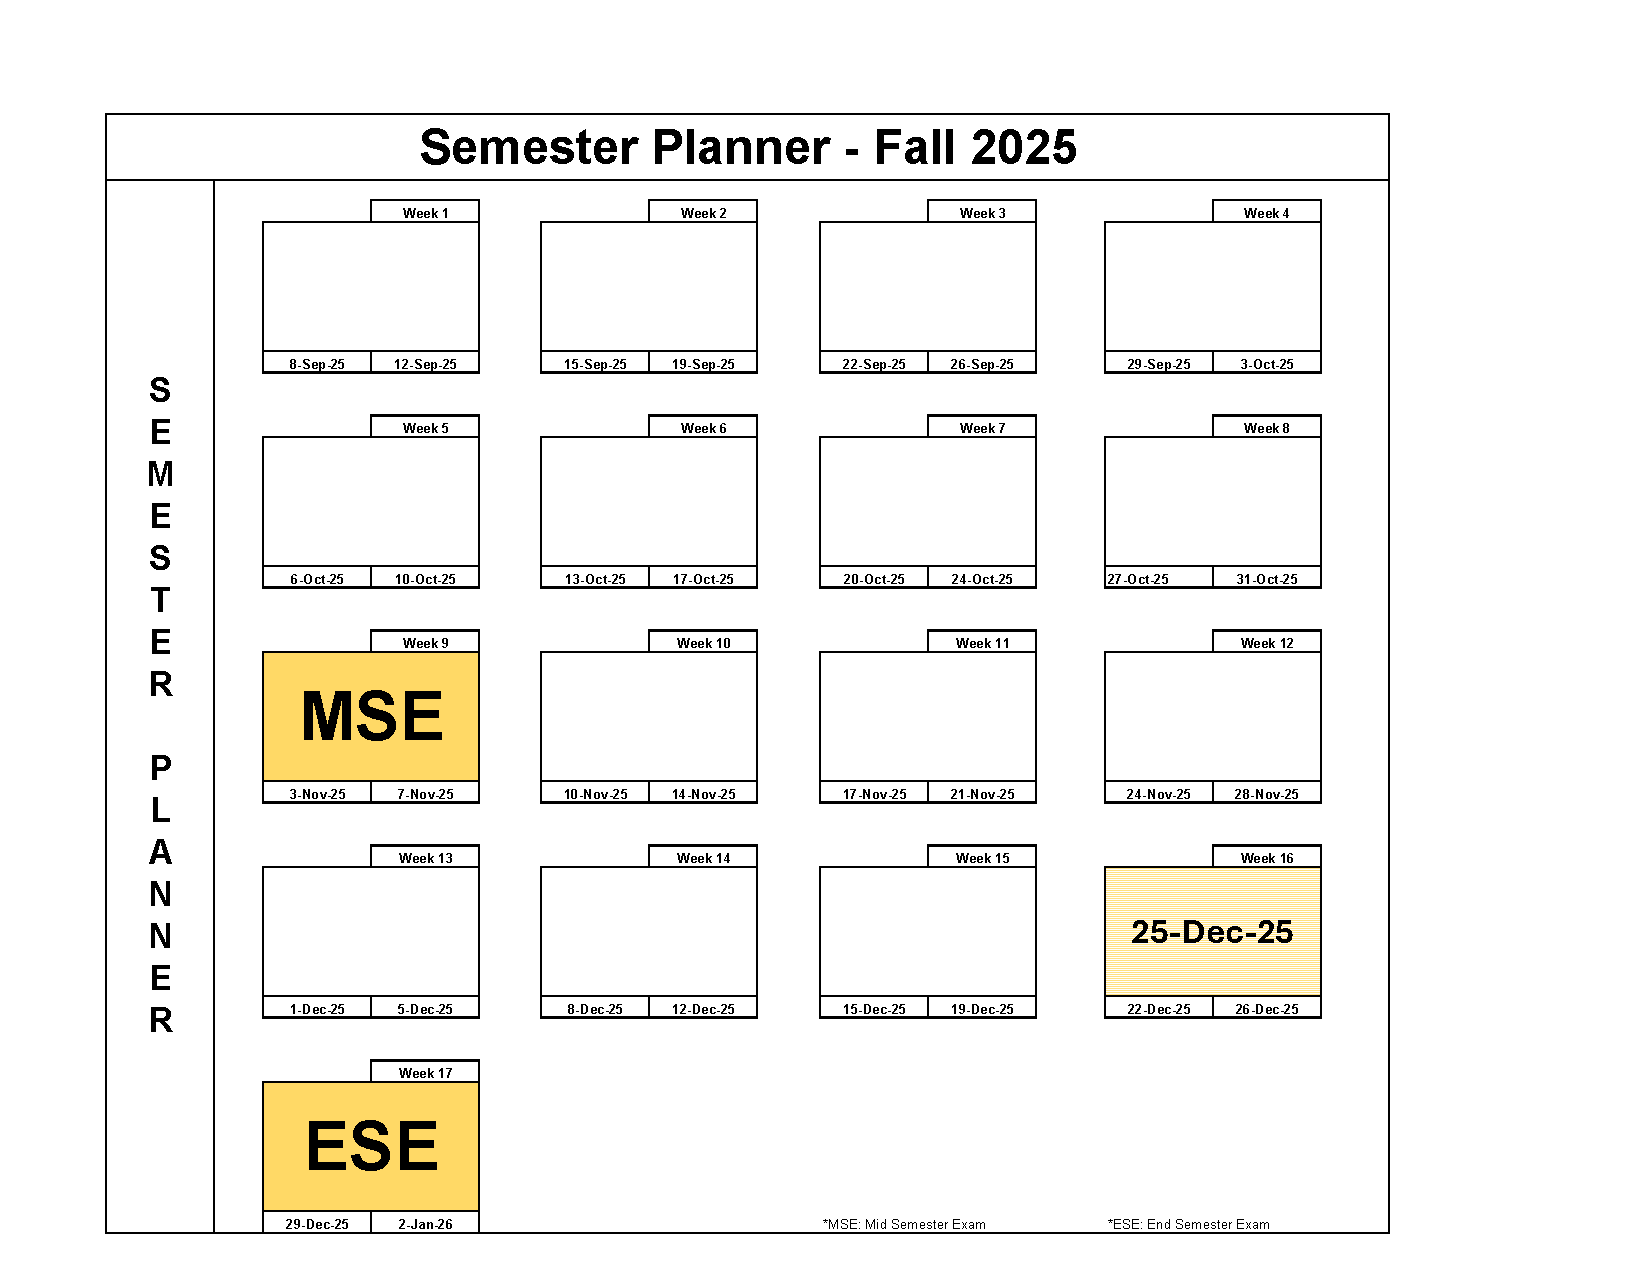
\includepdf[
  pages={1},
  scale=0.90,
  offset=0 -1.2cm,
  pagecommand={\thispagestyle{plain}\noindent{\Large\bfseries\thesection\quad Program Planning}}
]{appendices/criterion_8/I2.pdf}

\includepdf[
  pages={2-},
  pagecommand={\thispagestyle{plain}}
]{appendices/criterion_8/I2.pdf}

\refstepcounter{section}
\phantomsection
\label{annex:corrective}
\addcontentsline{toc}{section}{\protect\numberline{\thesection}Corrective Action Form}
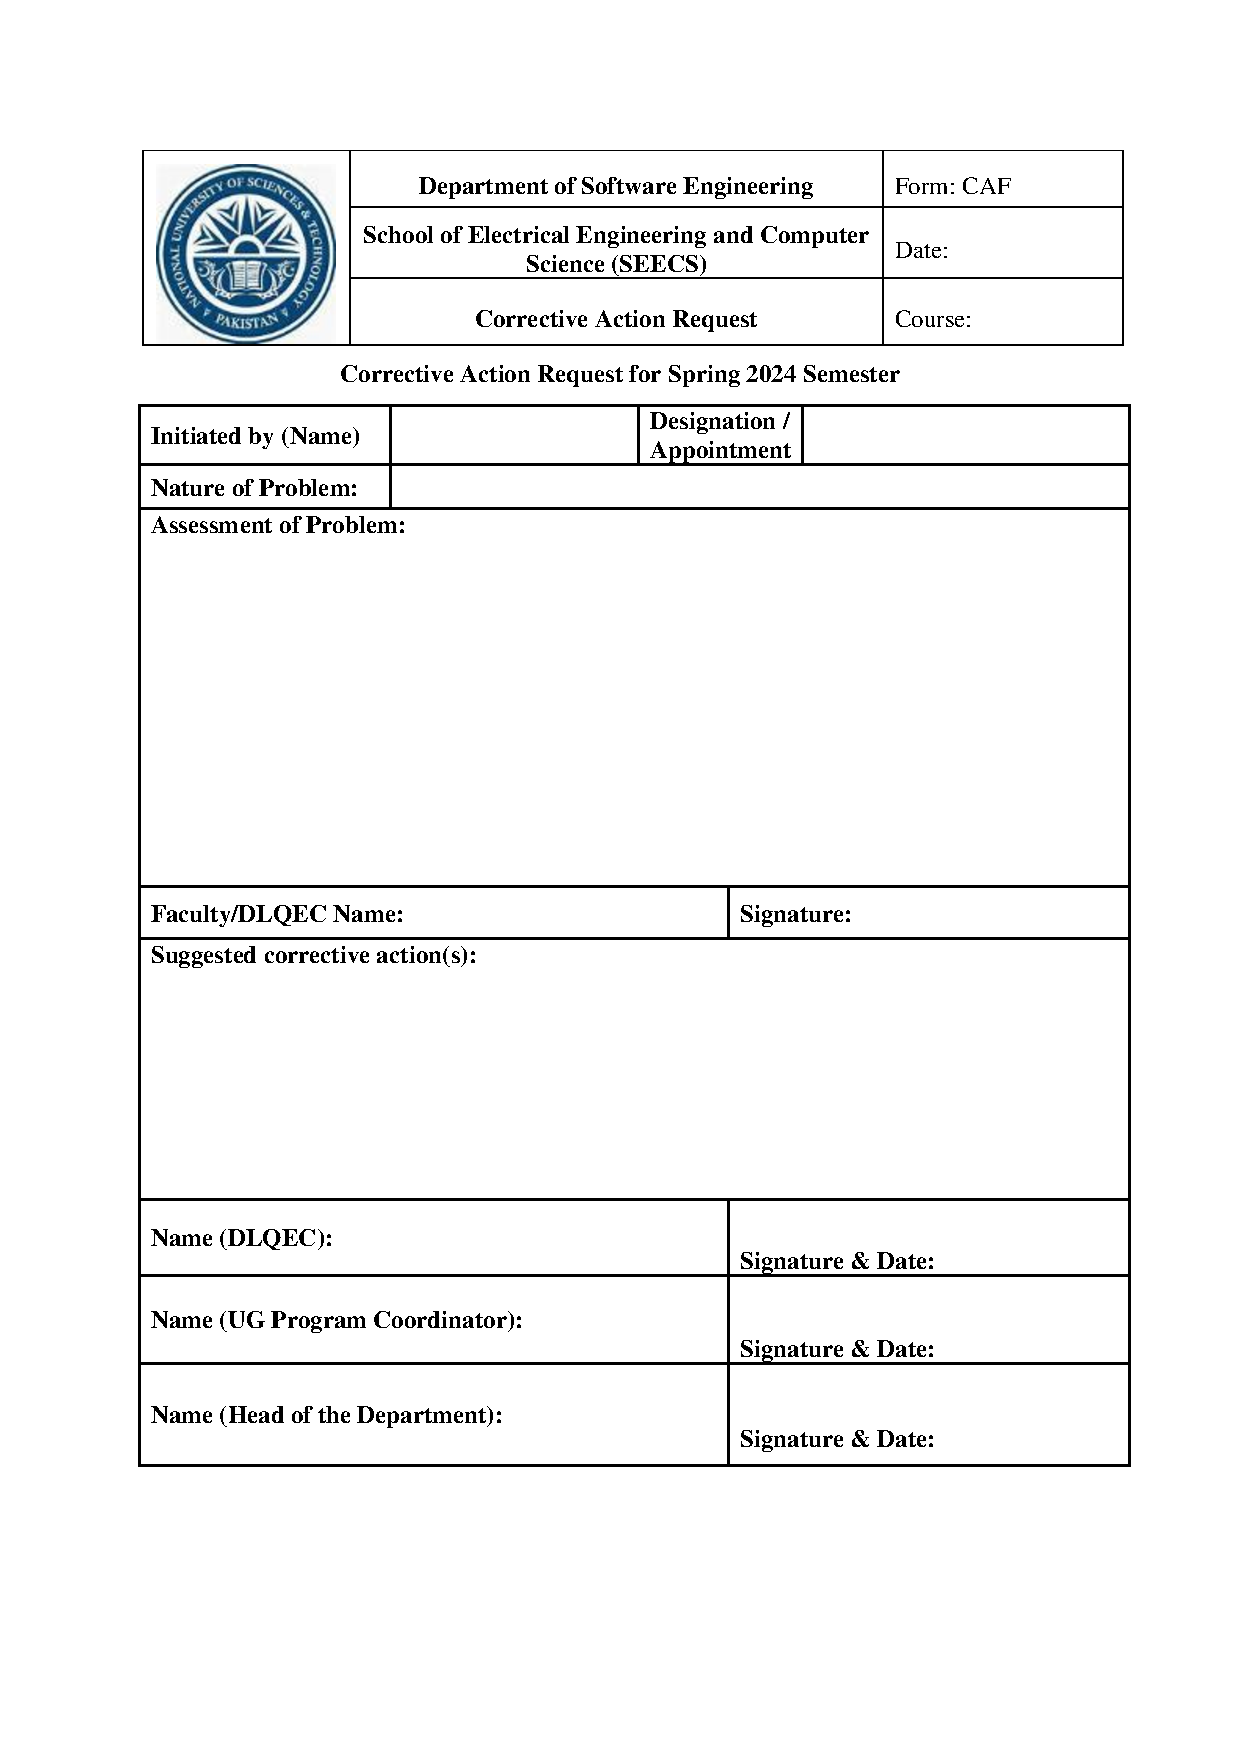
\includepdf[
  pages={1},
  scale=0.90,
  offset=0 -1.2cm,
  pagecommand={\thispagestyle{plain}\noindent{\Large\bfseries\thesection\quad Corrective Action Form}}
]{appendices/criterion_8/I3.pdf}

\refstepcounter{section}
\phantomsection
\label{annex:wp2024}
\addcontentsline{toc}{section}{\protect\numberline{\thesection}Working Paper for Curriculum Revision 2024}
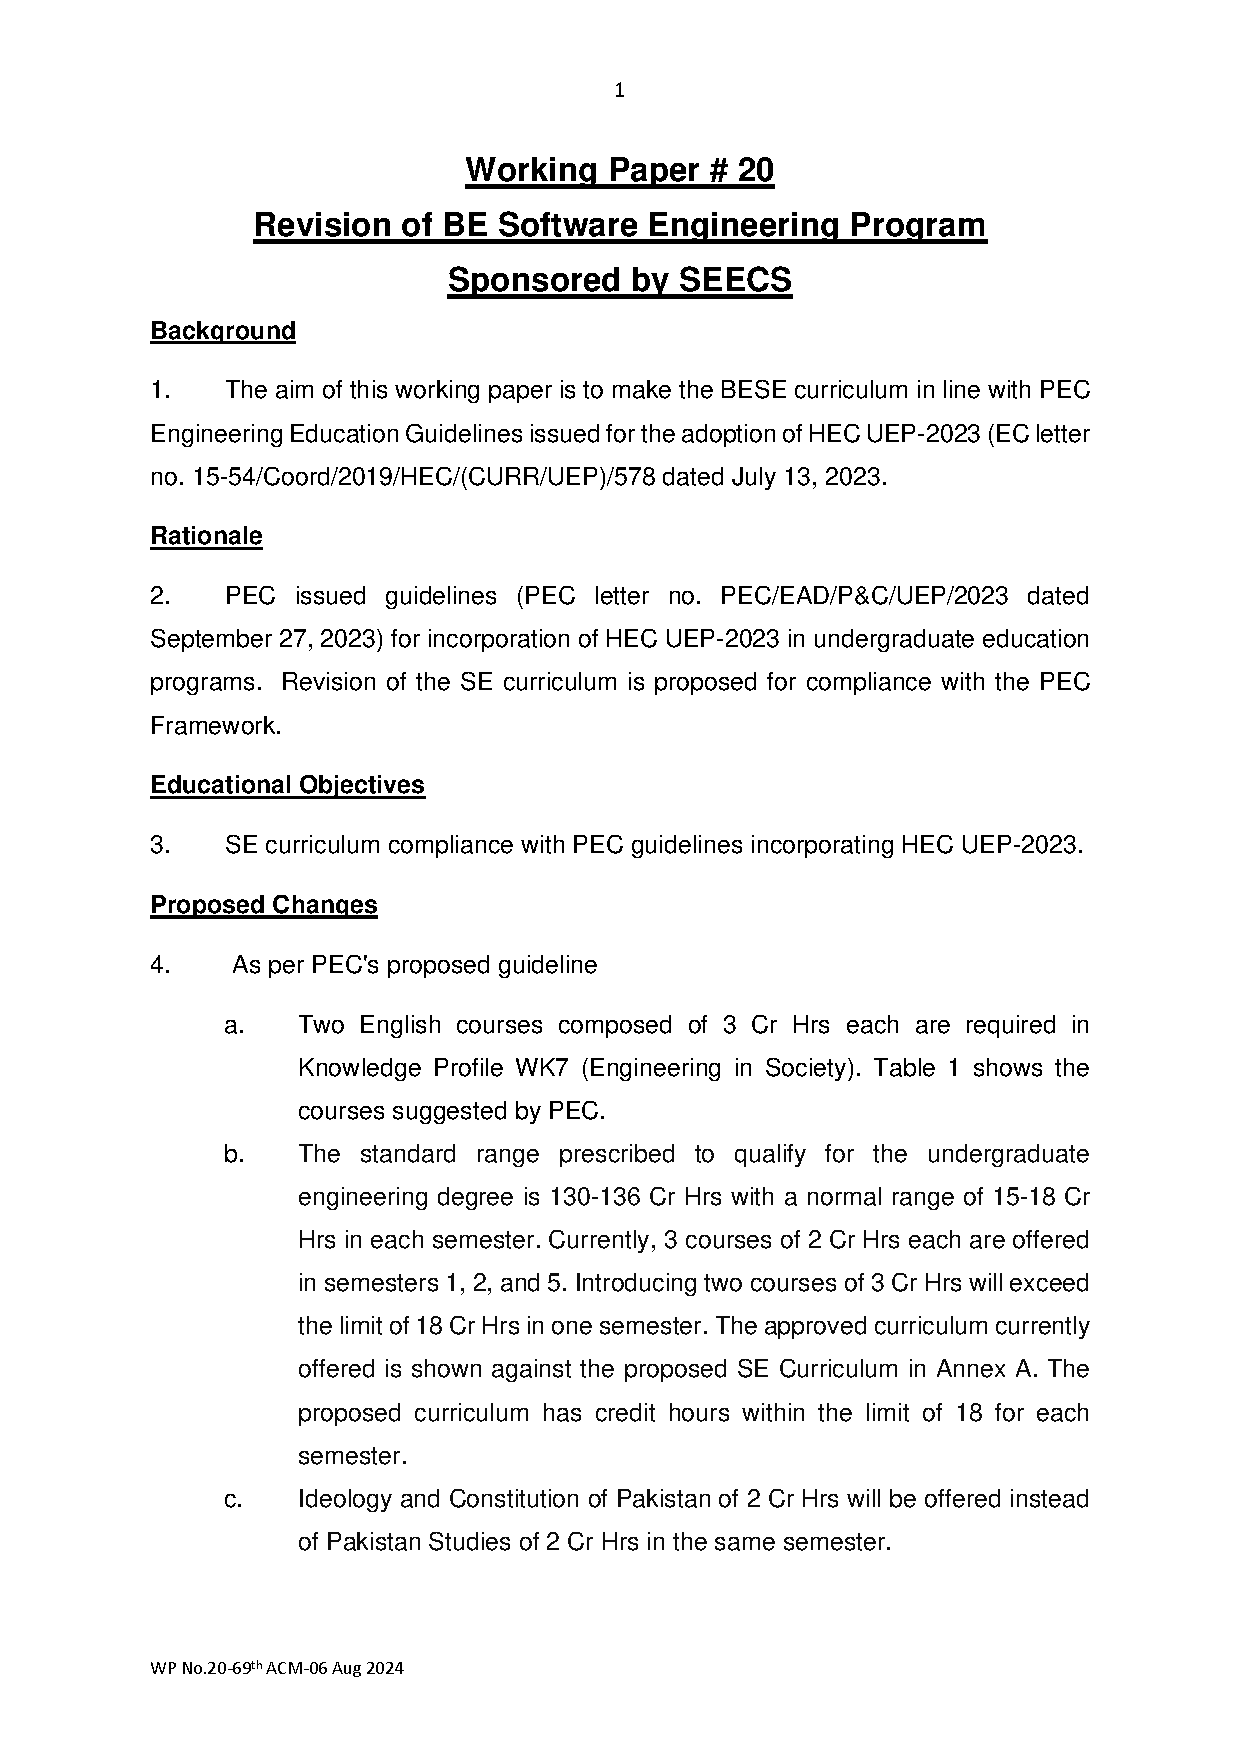
\includepdf[
  pages={1},
  scale=0.90,
  offset=0 -1.2cm,
  pagecommand={\thispagestyle{plain}\noindent{\Large\bfseries\thesection\quad Working Paper for Curriculum Revision 2024}}
]{appendices/criterion_3/Annex-2-WP-20-69-ACM-1-6.pdf}

\includepdf[
  pages={2-},
  pagecommand={\thispagestyle{plain}}
]{appendices/criterion_3/Annex-2-WP-20-69-ACM-1-6.pdf}

\refstepcounter{section}
\phantomsection
\label{annex:wp2025}
\addcontentsline{toc}{section}{\protect\numberline{\thesection}Working Paper for Curriculum Revision 2025}
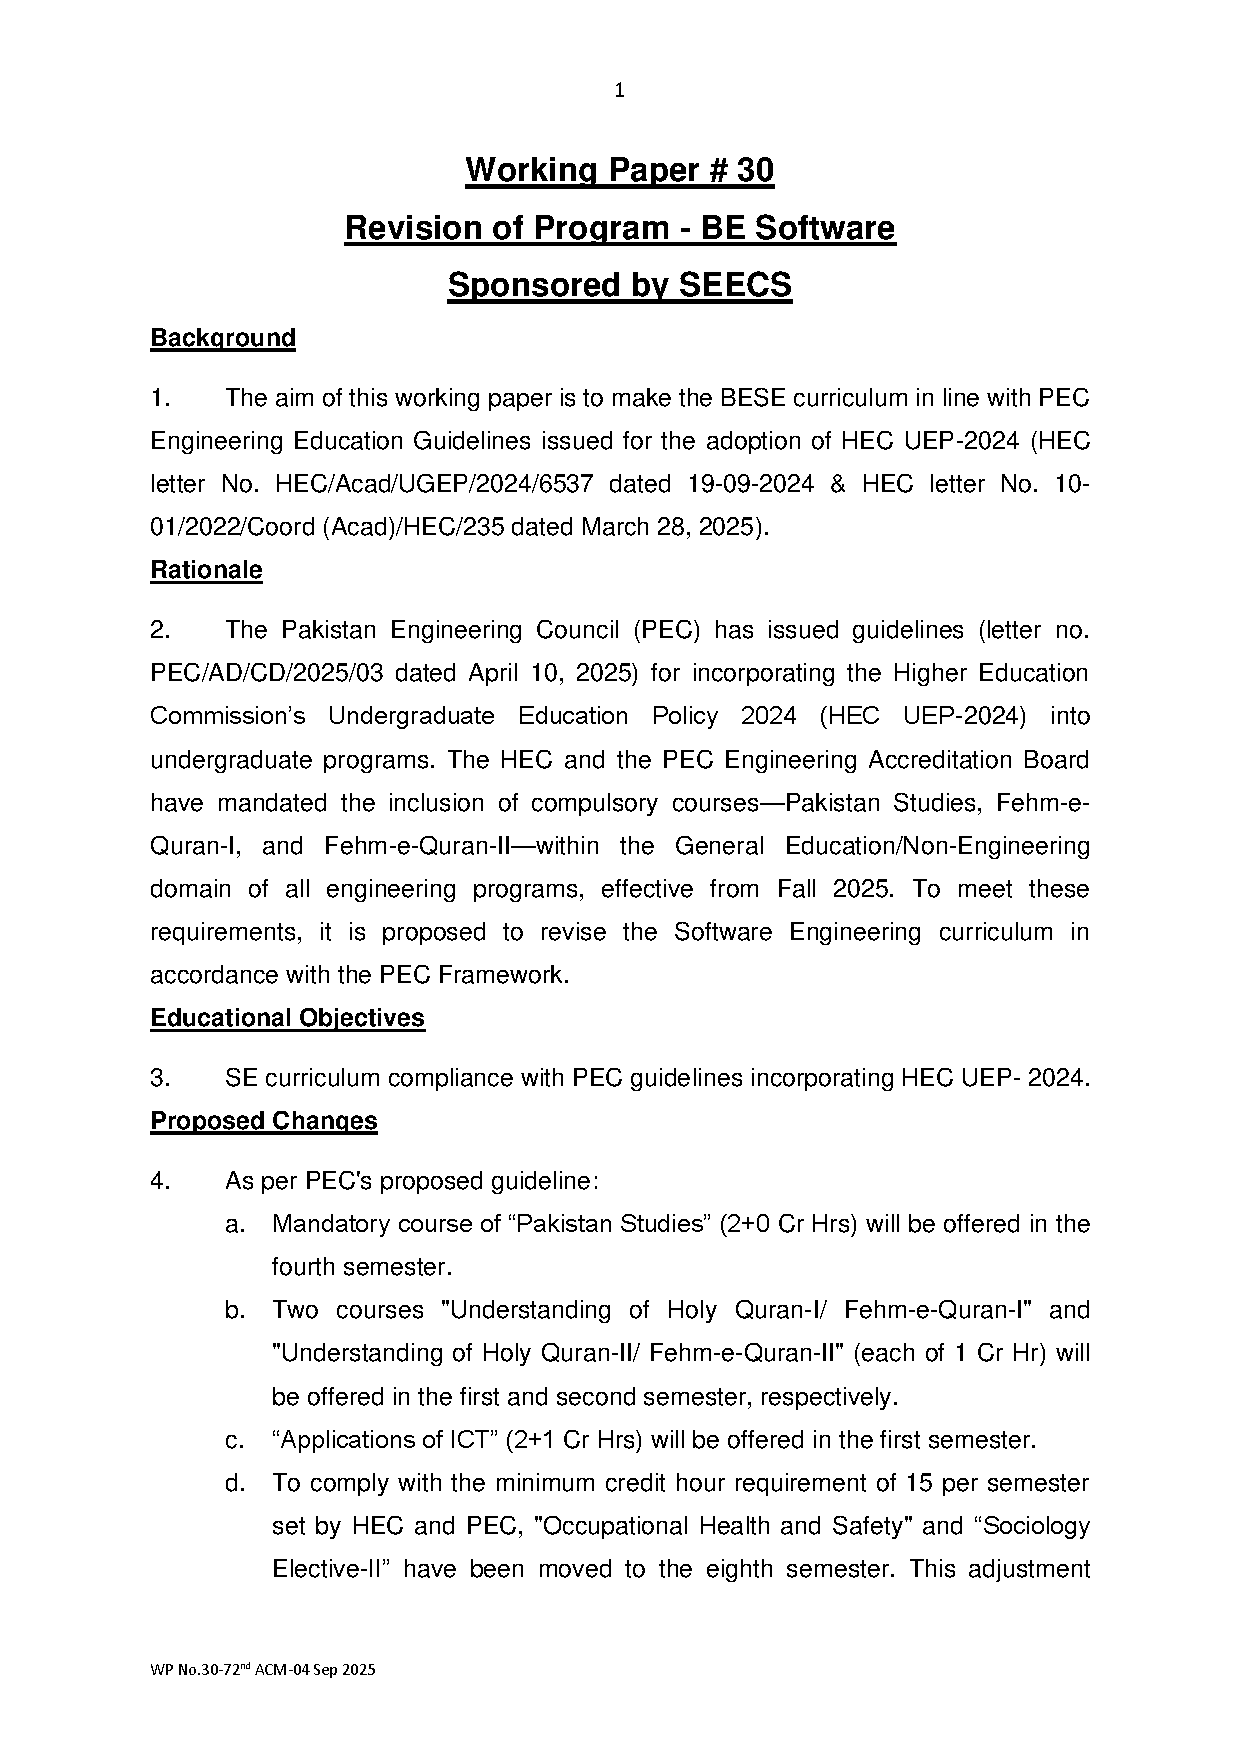
\includepdf[
  pages={1},
  scale=0.90,
  offset=0 -1.2cm,
  pagecommand={\thispagestyle{plain}\noindent{\Large\bfseries\thesection\quad Working Paper for Curriculum Revision 2025}}
]{appendices/criterion_3/Annex-1-WP-30-72-ACM.pdf}

\includepdf[
  pages={2-},
  pagecommand={\thispagestyle{plain}}
]{appendices/criterion_3/Annex-1-WP-30-72-ACM.pdf}


\refstepcounter{section}
\phantomsection
\label{annex:alumni}
\addcontentsline{toc}{section}{\protect\numberline{\thesection}Alumni Survey Form}
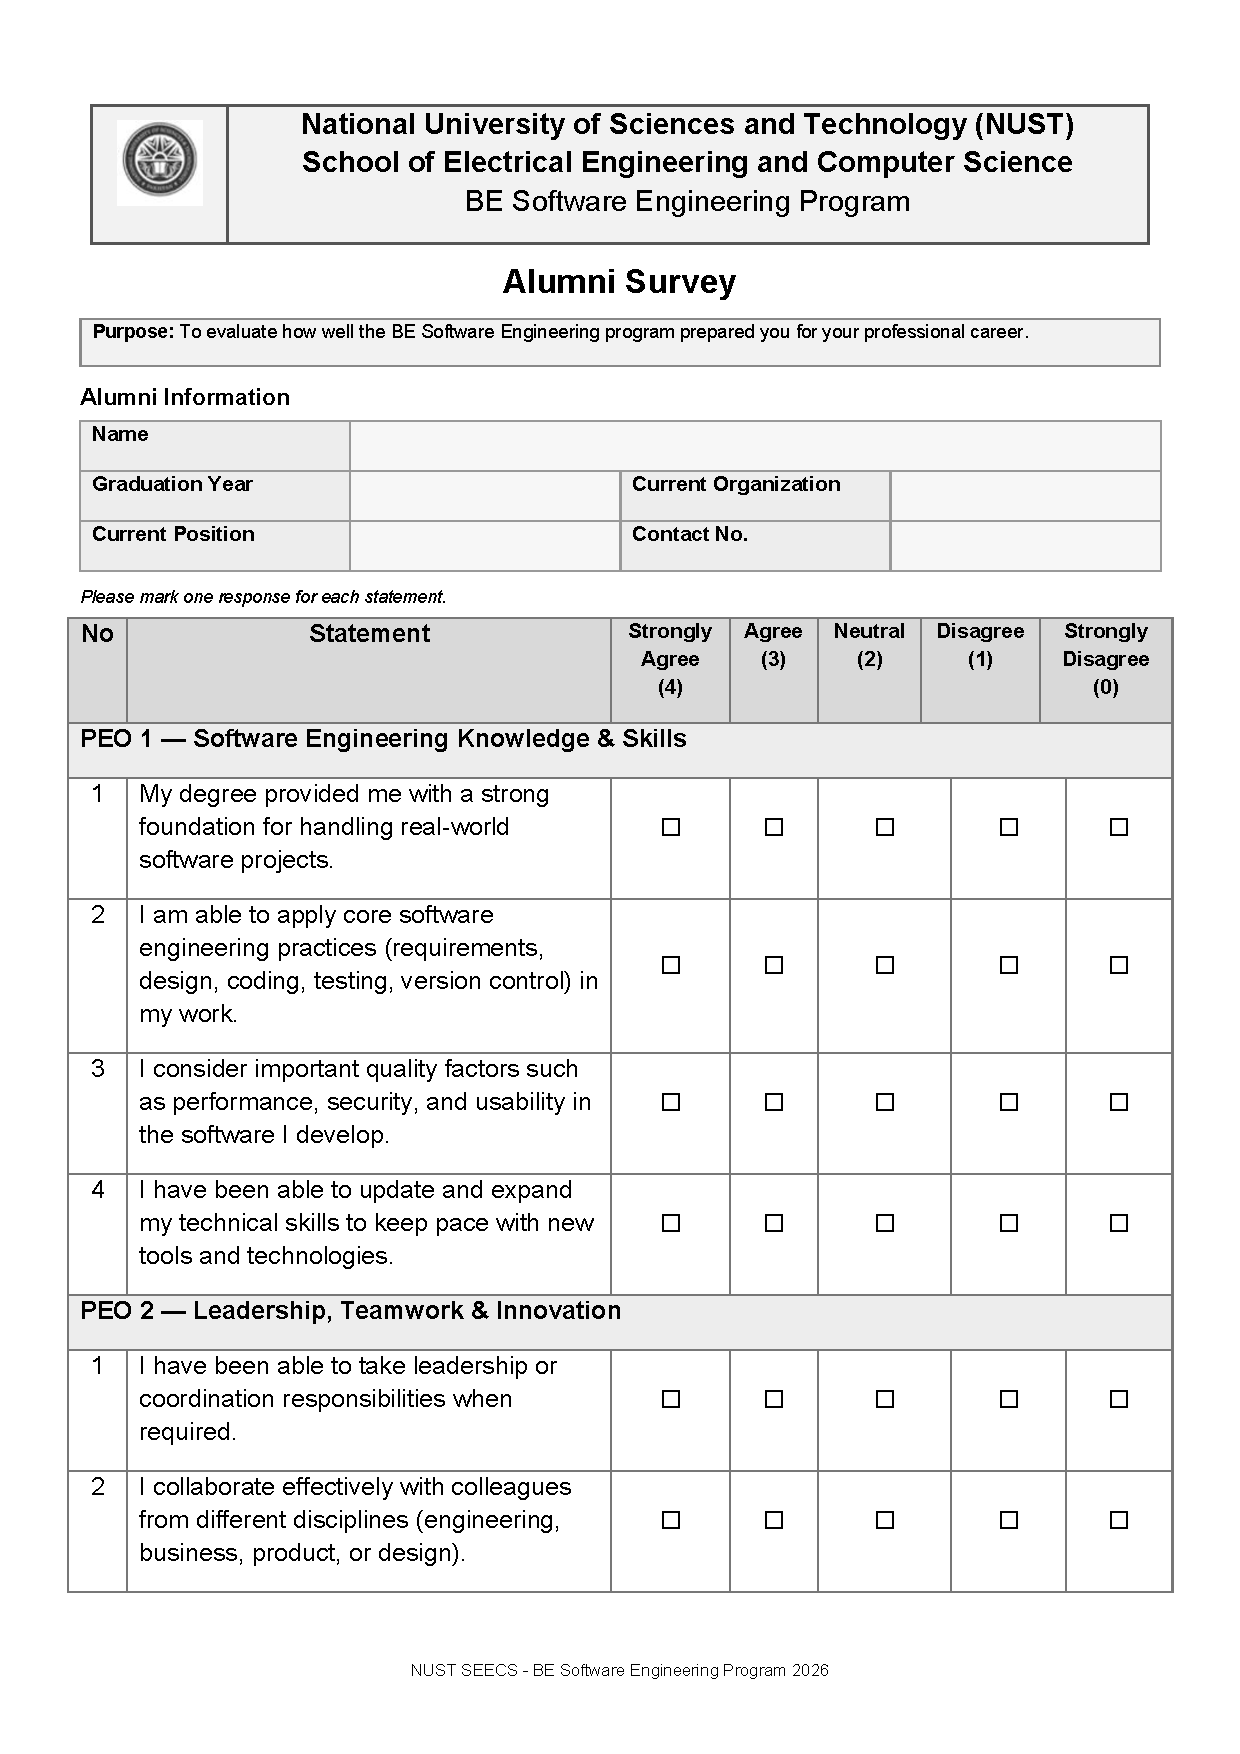
\includepdf[
  pages={1},
  scale=0.90,
  offset=0 -1.2cm,
  pagecommand={\thispagestyle{plain}\noindent{\Large\bfseries\thesection\quad Alumni Survey Form}}
]{appendices/criterion_1/Alumni Survey 2026.pdf}

\includepdf[
  pages={2-},
  pagecommand={\thispagestyle{plain}}
]{appendices/criterion_1/Alumni Survey 2026.pdf}


\refstepcounter{section}
\phantomsection
\label{annex:employer}
\addcontentsline{toc}{section}{\protect\numberline{\thesection}Employer Survey Form}
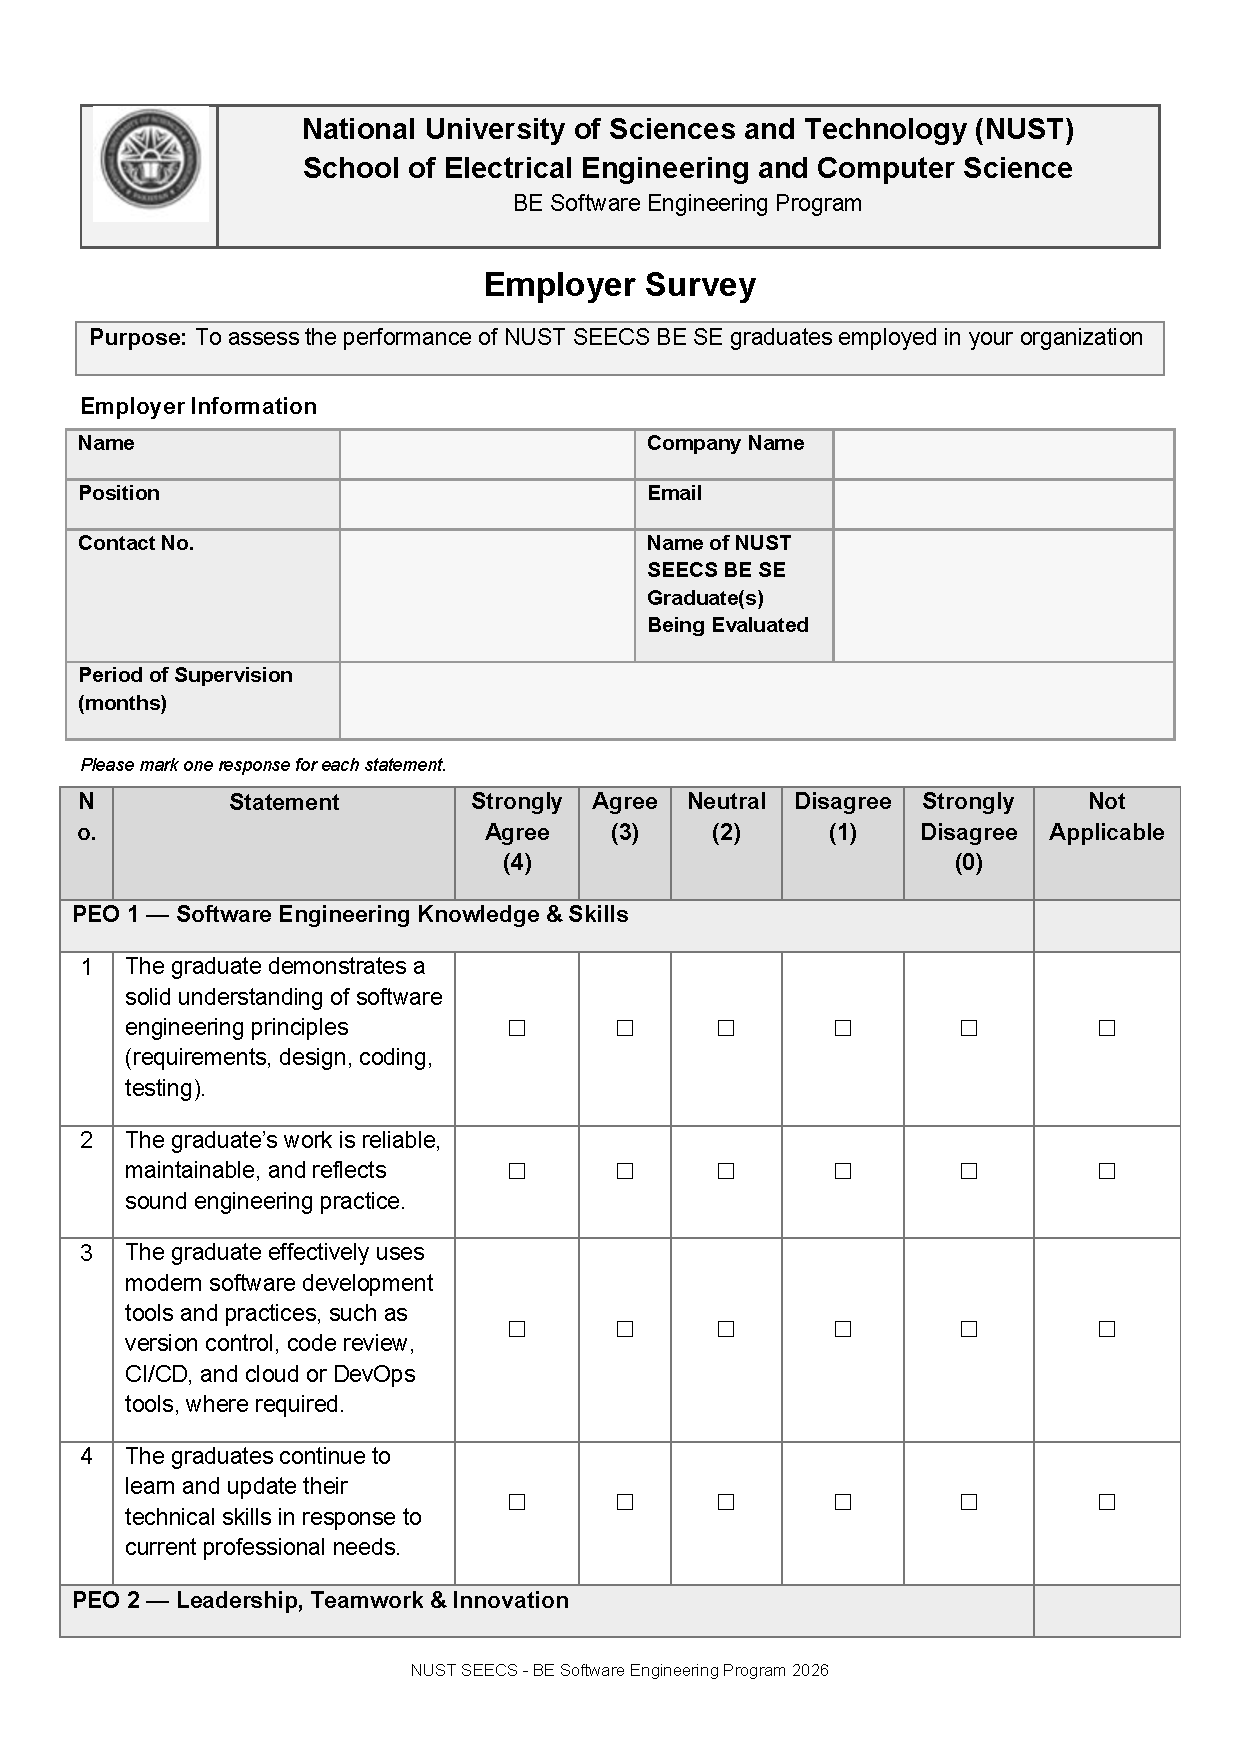
\includepdf[
  pages={1},
  scale=0.90,
  offset=0 -1.2cm,
  pagecommand={\thispagestyle{plain}\noindent{\Large\bfseries\thesection\quad Employer Survey Form}}
]{appendices/criterion_1/Employer Survey 2026.pdf}

\includepdf[
  pages={2-},
  pagecommand={\thispagestyle{plain}}
]{appendices/criterion_1/Employer Survey 2026.pdf}

\refstepcounter{section}
\phantomsection
\label{annex:advice}
\addcontentsline{toc}{section}{\protect\numberline{\thesection}Letter of Advice}
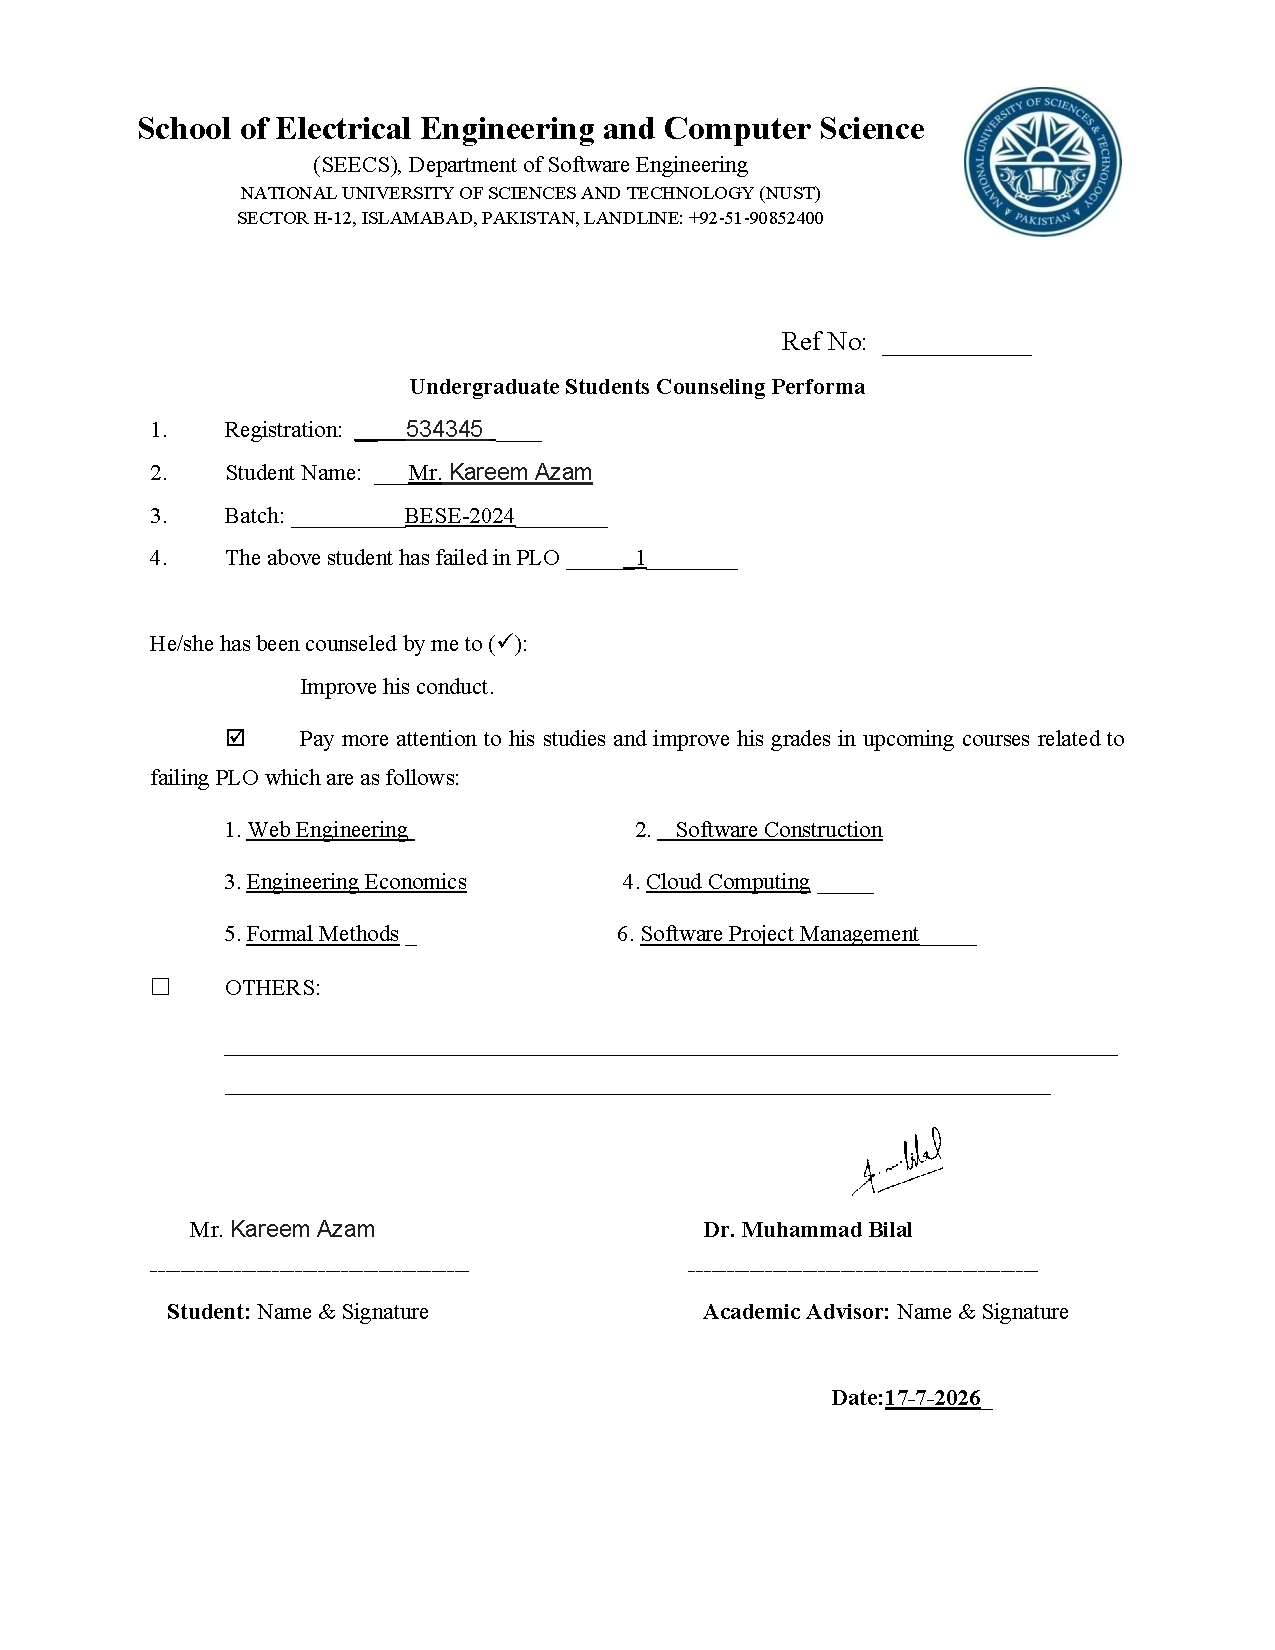
\includepdf[
  pages={1},
  scale=0.90,
  offset=0 -1.2cm,
  pagecommand={\thispagestyle{plain}\noindent{\Large\bfseries\thesection\quad Letter of Advice}}
]{appendices/criterion_8/I7.pdf}


\refstepcounter{section}
\phantomsection
\label{annex:oop}
\addcontentsline{toc}{section}{\protect\numberline{\thesection}CQI Form Sample}
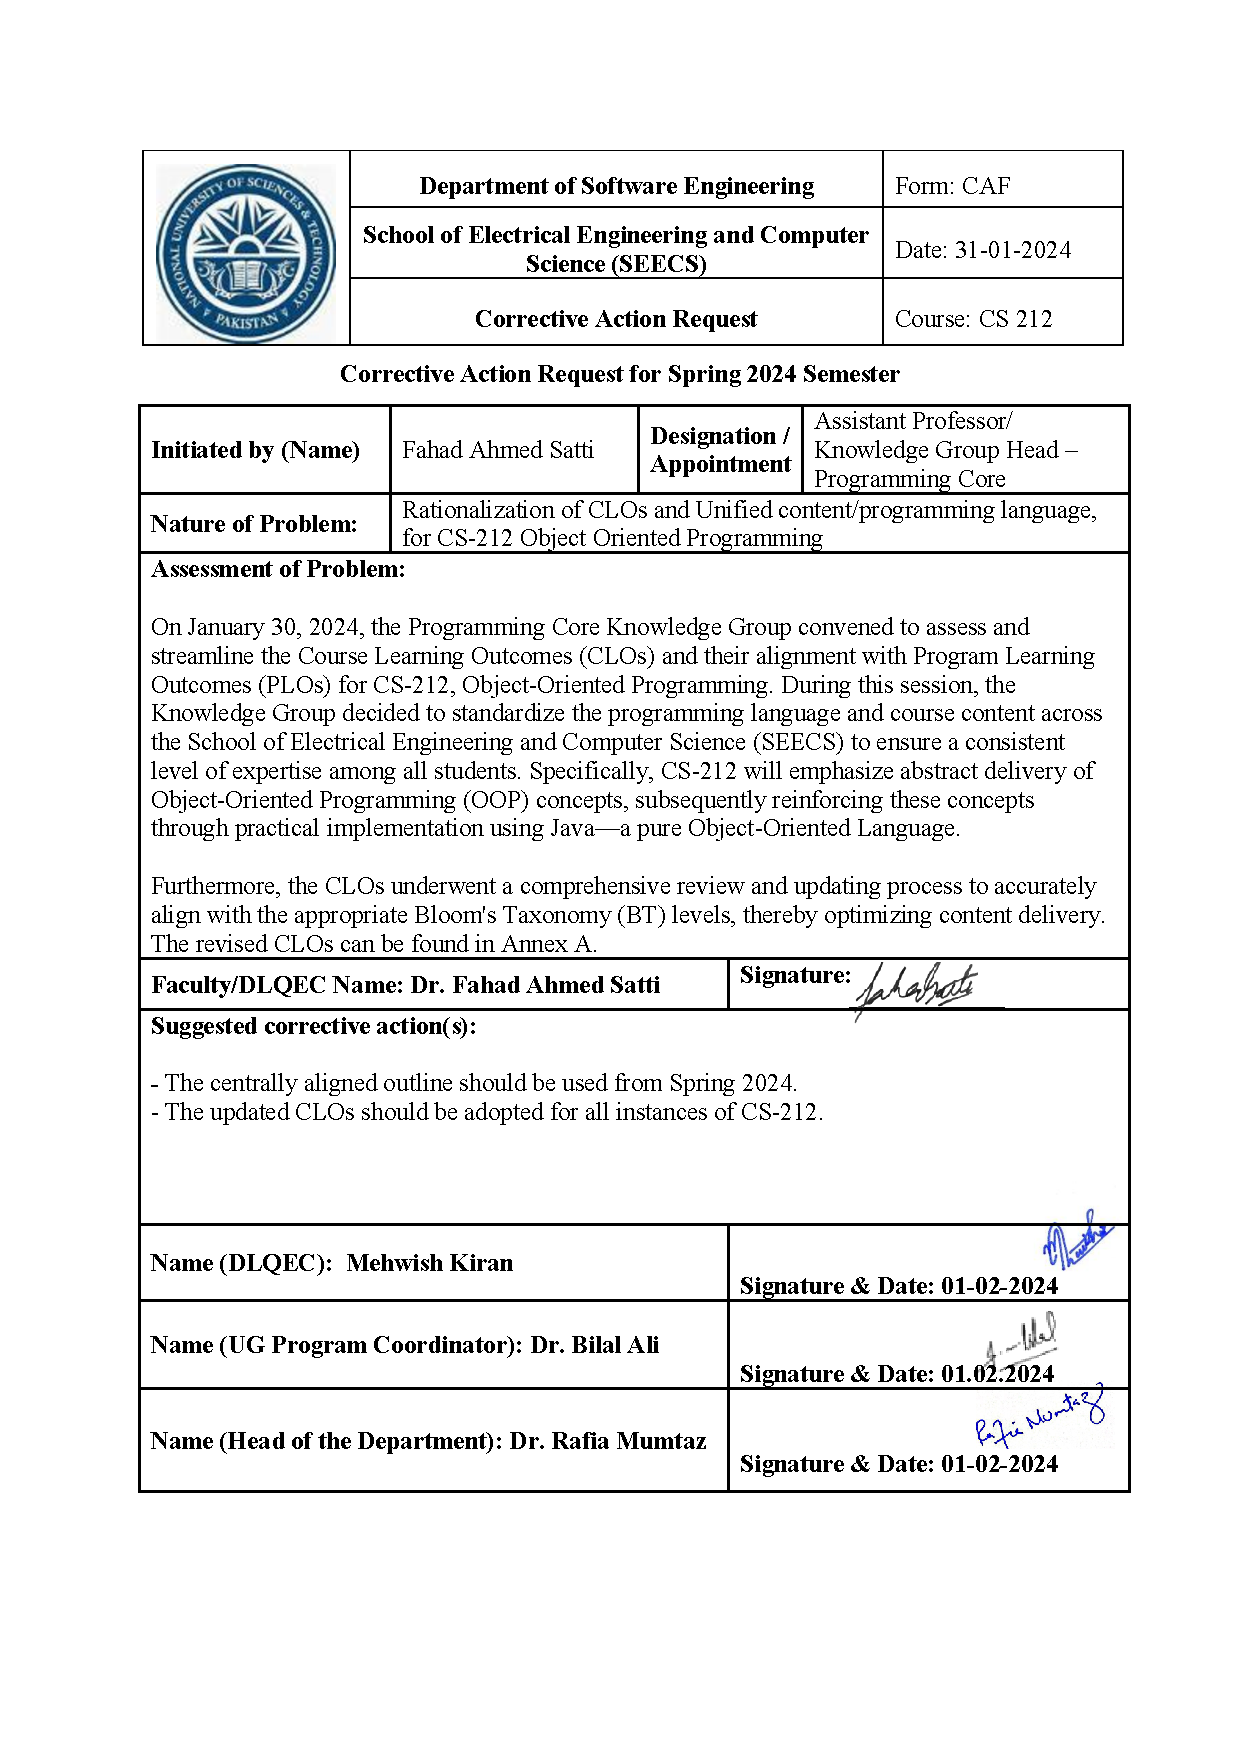
\includepdf[
  pages={1},
  scale=0.90,
  offset=0 -1.2cm,
  pagecommand={\thispagestyle{plain}\noindent{\Large\bfseries\thesection\quad CQI Form Sample}}
]{appendices/criterion_8/I8.pdf}

\includepdf[
  pages={2-},
  pagecommand={\thispagestyle{plain}}
]{appendices/criterion_8/I8.pdf}
